%
% main.tex -- Paper zum Thema <rossby>
%
% (c) 2020 Autor, OST Ostschweizer Fachhochschule
%
% !TEX root = ../../buch.tex
% !TEX encoding = UTF-8
% !TeX spellcheck = de-CH

\chapter{Rossby Wellen\label{chapter:rossby}}
\kopflinks{Rossby Wellen}
\begin{refsection}
	\chapterauthor{Michael Schmid}


    \section{Einleitung}

    Schon im frühen 20. Jahrhundert begannen Meteorologinnen und Meteorologen zu erkennen, dass grossräumige Strömungen in der Atmosphäre nicht nur durch Temperaturunterschiede, sondern auch durch die Erdrotation beeinflusst werden.  
    Eine Schlüsselfigur in diesem Zusammenhang war Carl-Gustaf Rossby, ein schwedisch-amerikanischer Meteorologe.  
    In seiner Arbeit von 1939 untersuchte er den Zusammenhang zwischen der Intensität der zonalen Zirkulation und der Verschiebung der sogenannten permanenten Aktionszentren in der Atmosphäre \cite{rossby:1939relation}.  
    Ein Jahr später veröffentlichte er seine grundlegende Theorie der planetaren Wellenmuster in der Atmosphäre, die heute als \emph{Rossby-Wellen} bekannt sind \cite{rossby:1940planetary}.  
    Diese Wellen sind heute ein zentrales Konzept in der Dynamik der Atmosphäre und tragen wesentlich zum Verständnis des Wetters in den mittleren Breiten bei.  
    
    Rossby erkannte, dass die scheinbaren Kräfte, die durch die Rotation der Erde entstehen - insbesondere der \emph{Coriolis-Effekt} -, eine wellenartige Bewegung grossräumiger atmosphärischer Strömungen erzeugen können.  
    Diese wellenförmigen Muster bewegen sich typischerweise von West nach Ost und beeinflussen massgeblich Hoch- und Tiefdrucksysteme sowie den Verlauf von Wetterfronten über Tage hinweg.  
    
    Die Untersuchung dieser Prozesse erfordert ein Verständnis physikalischer Konzepte wie der \emph{Vorticity} (Wirbelstärke), der \emph{absoluten} und \emph{potenziellen Vorticity} sowie deren Erhaltung unter bestimmten Bedingungen.  
    Diese Begriffe ermöglichen es, die Bewegung von Luftpaketen auf einem rotierenden Planeten mathematisch zu beschreiben und zu erklären, warum Rossby-Wellen entstehen und wie sie sich ausbreiten.  
    
    Ziel dieses Textes ist es, die Grundlagen der atmosphärischen Dynamik zu skizzieren, die zur Entstehung von Rossby-Wellen führen.  
    Beginnend mit der Erddrehung und dem Coriolis-Effekt, werden die Begriffe der Vorticity eingeführt und schrittweise zur potenziellen Vorticity erweitert.  
    Die Erhaltung dieser Grösse stellt den Ausgangspunkt für die mathematische Herleitung und das physikalische Verständnis von Rossby-Wellen dar.  
    Abschliessend wird ihre Rolle in typischen Wetterphänomenen beleuchtet.  
    

    \section{Visuelle Einführung: Rossby-Wellen im Wettergeschehen}

    Eine Folge von Karten der 500\,hPa-Höhenfelder und Windgeschwindigkeiten zeigt deutlich die Dynamik und wellenartige Struktur der Rossby-Wellen im Zeitraum vom 1. bis 10. Mai 2025.  
    Die Wellenmuster bewegen sich von West nach Ost, wobei Hoch- und Tiefdruckgebiete mit den Wellenbergen und -tälern korrespondieren.  
    Diese Visualisierung vermittelt ein intuitives Verständnis für die grossräumigen atmosphärischen Prozesse, die in den folgenden Abschnitten mathematisch und physikalisch analysiert werden.  
    Die vollständige Sequenz ist in der begleitenden Präsentation enthalten.  


    \begin{figure}
        \centering
        \renewcommand{\arraystretch}{0.5}
        \begin{tabular}{ccc}
            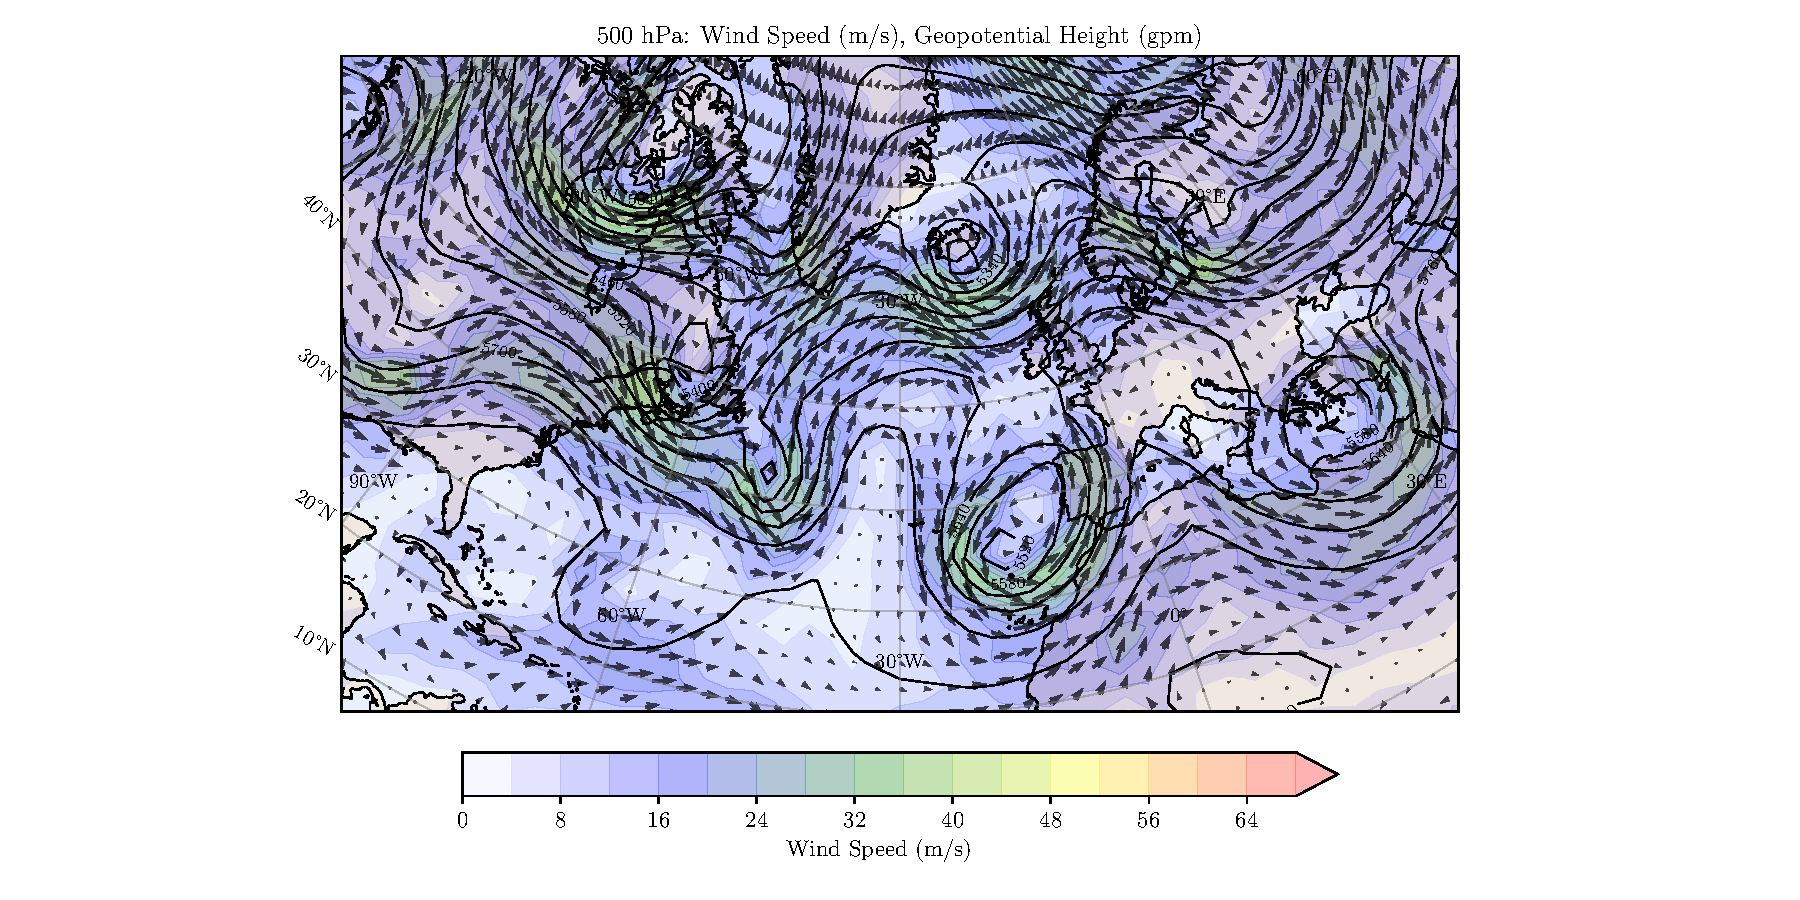
\includegraphics[width=0.32\textwidth, trim=5cm 0cm 5cm 0cm, clip]{papers/rossby/images/weather/data_2025_5_1_00:00_500.pdf} &
            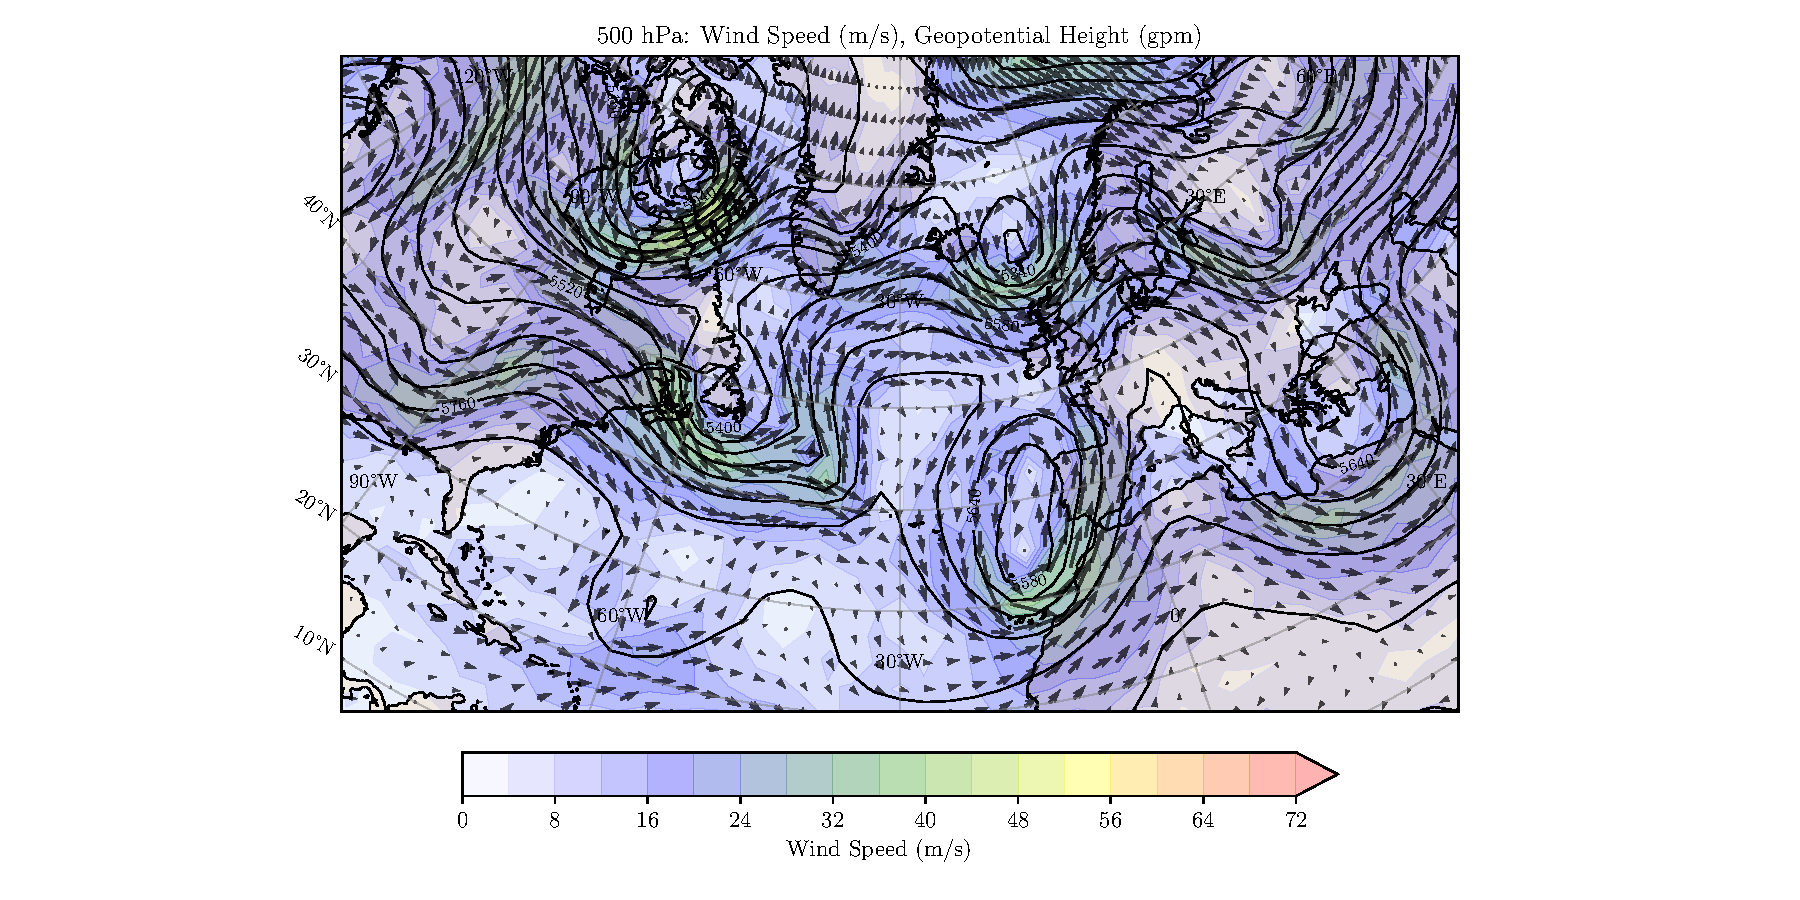
\includegraphics[width=0.32\textwidth, trim=5cm 0cm 5cm 0cm, clip]{papers/rossby/images/weather/data_2025_5_1_12:00_500.pdf} &
            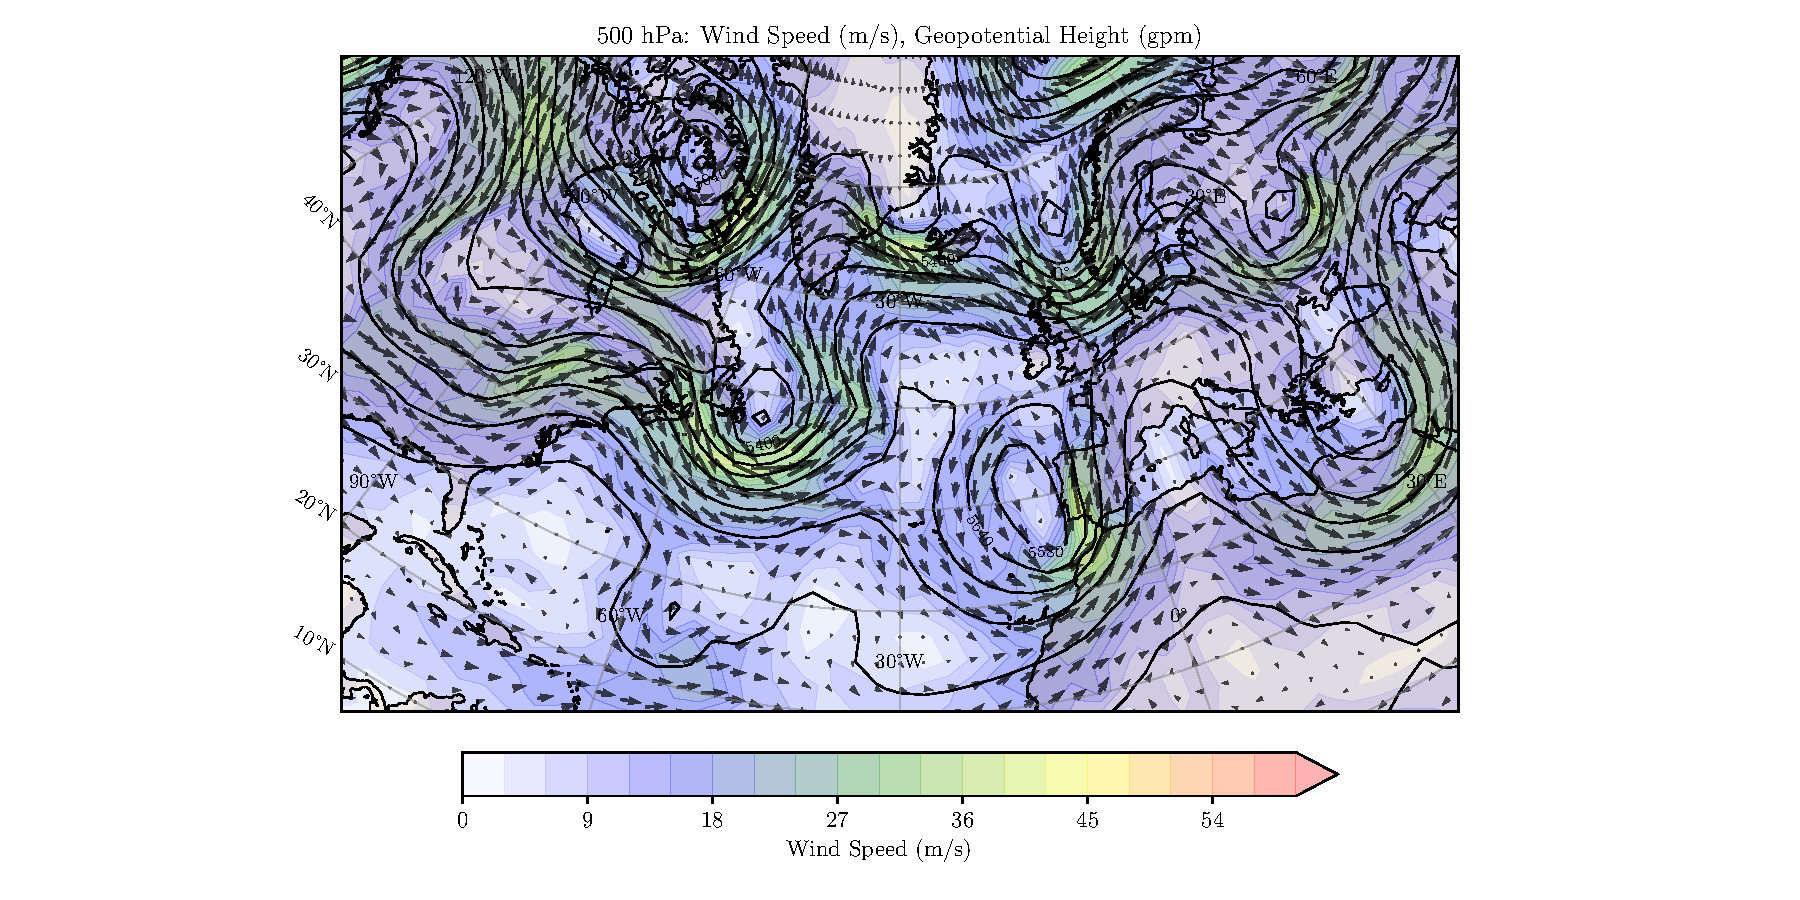
\includegraphics[width=0.32\textwidth, trim=5cm 0cm 5cm 0cm, clip]{papers/rossby/images/weather/data_2025_5_2_00:00_500.pdf} \\
            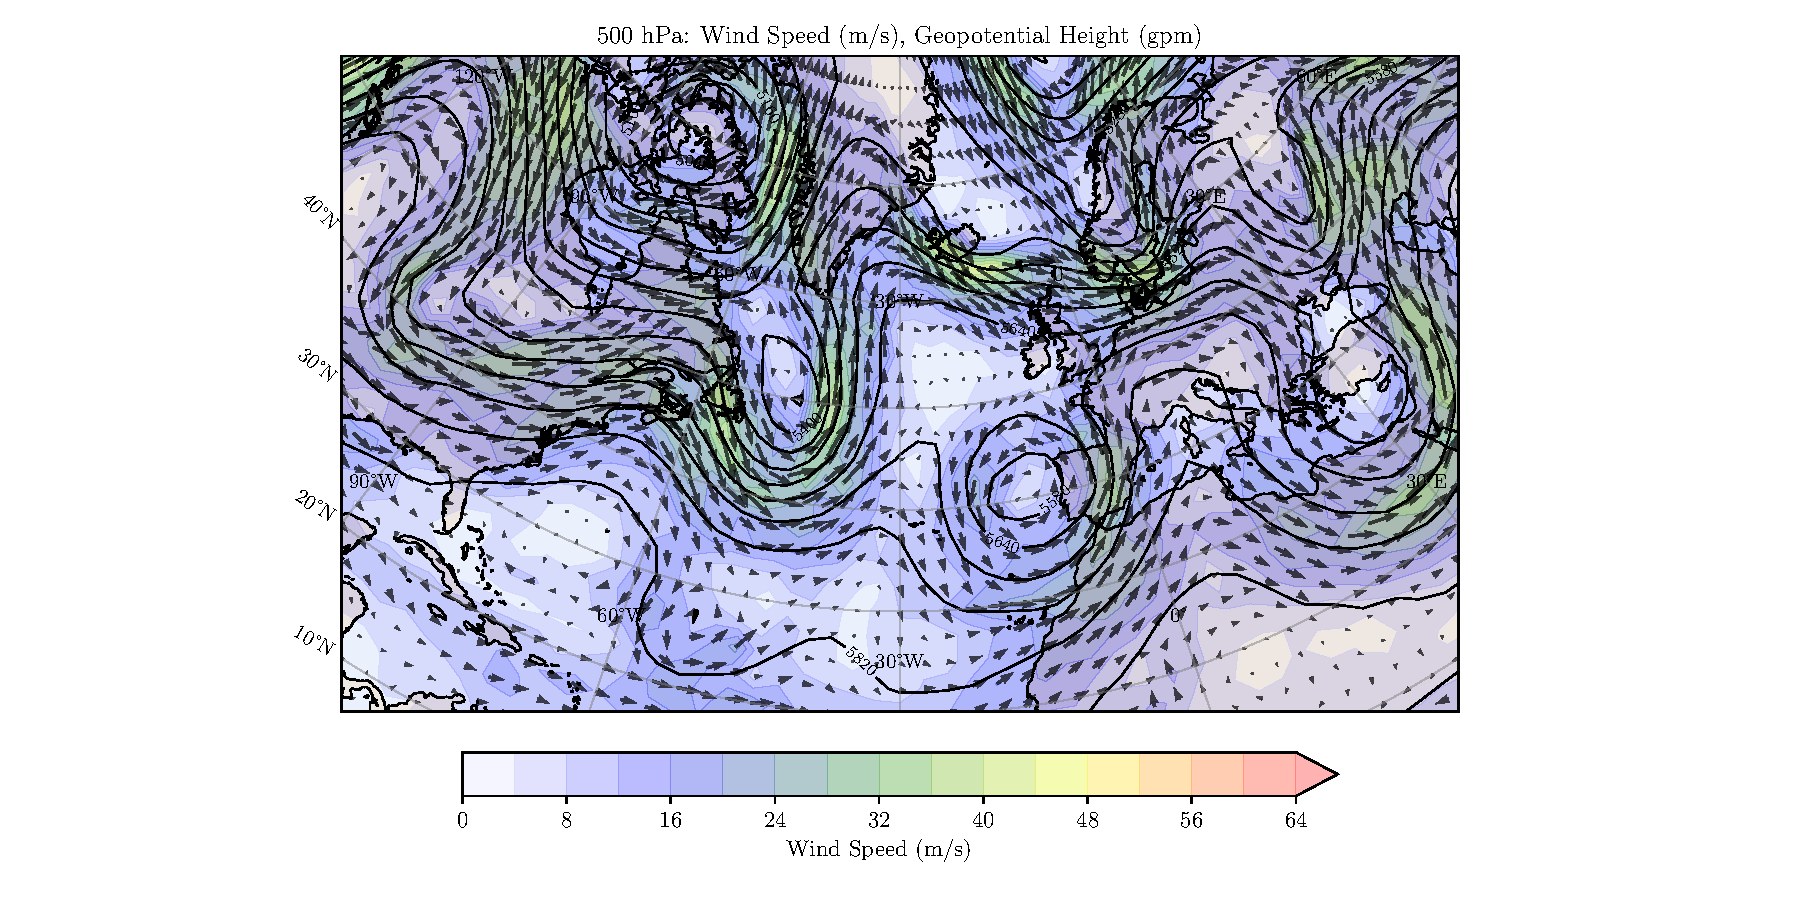
\includegraphics[width=0.32\textwidth, trim=5cm 0cm 5cm 0cm, clip]{papers/rossby/images/weather/data_2025_5_2_12:00_500.pdf} &
            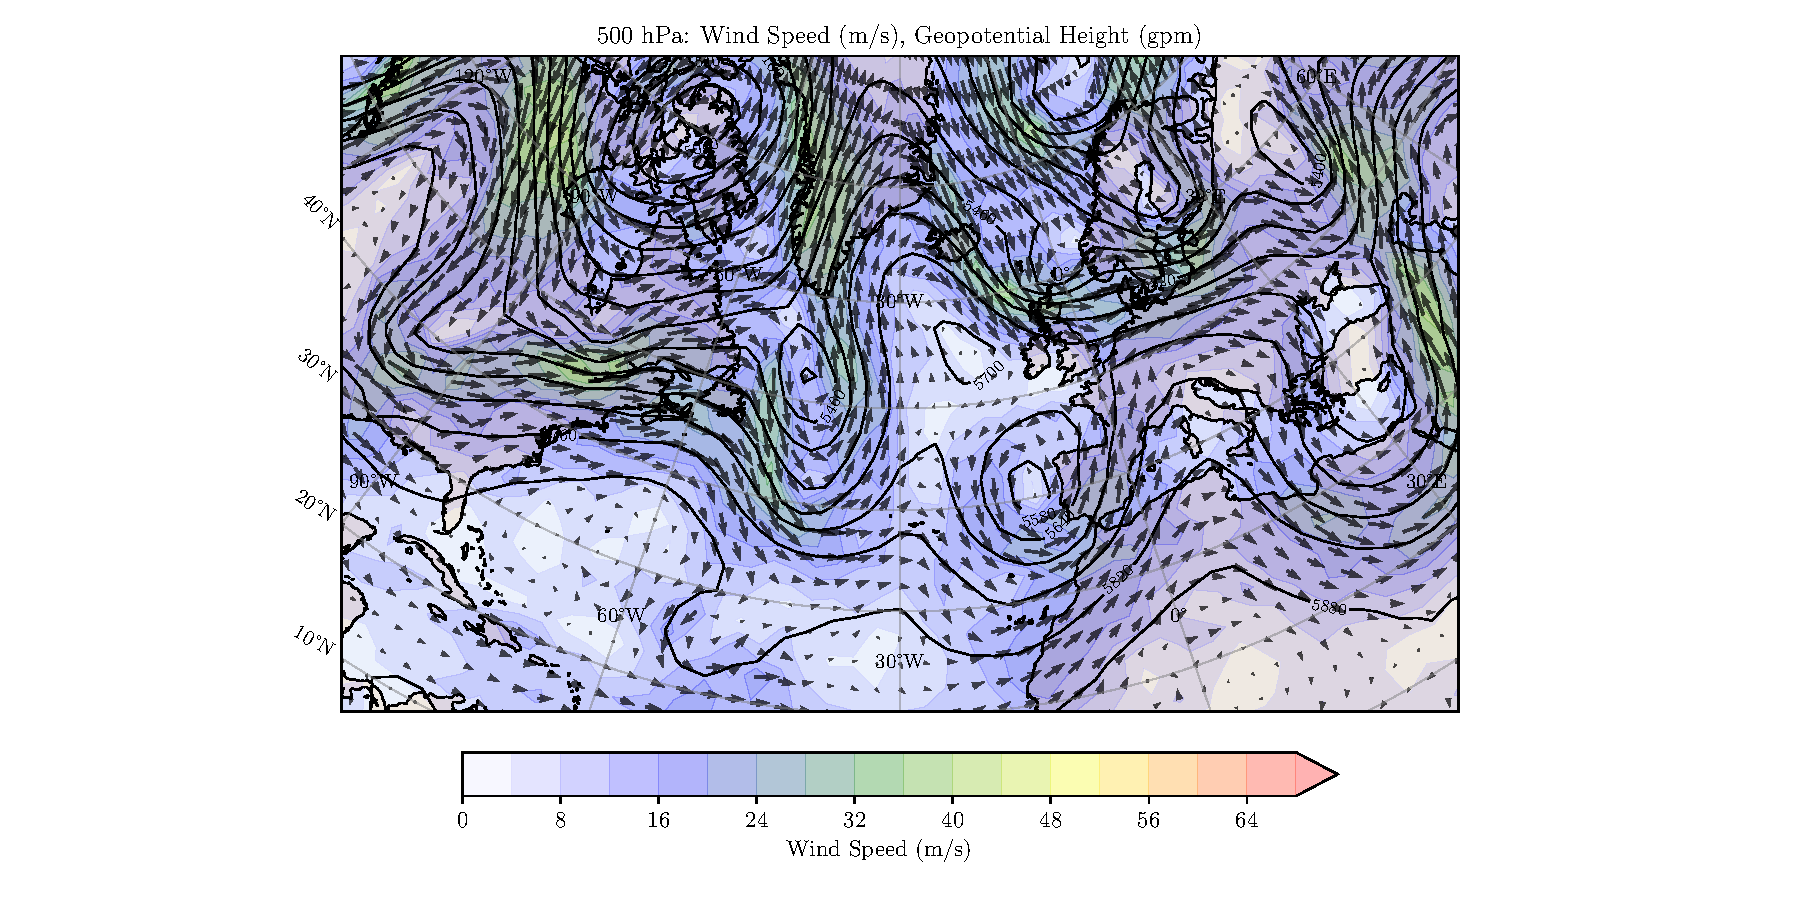
\includegraphics[width=0.32\textwidth, trim=5cm 0cm 5cm 0cm, clip]{papers/rossby/images/weather/data_2025_5_3_00:00_500.pdf} &
            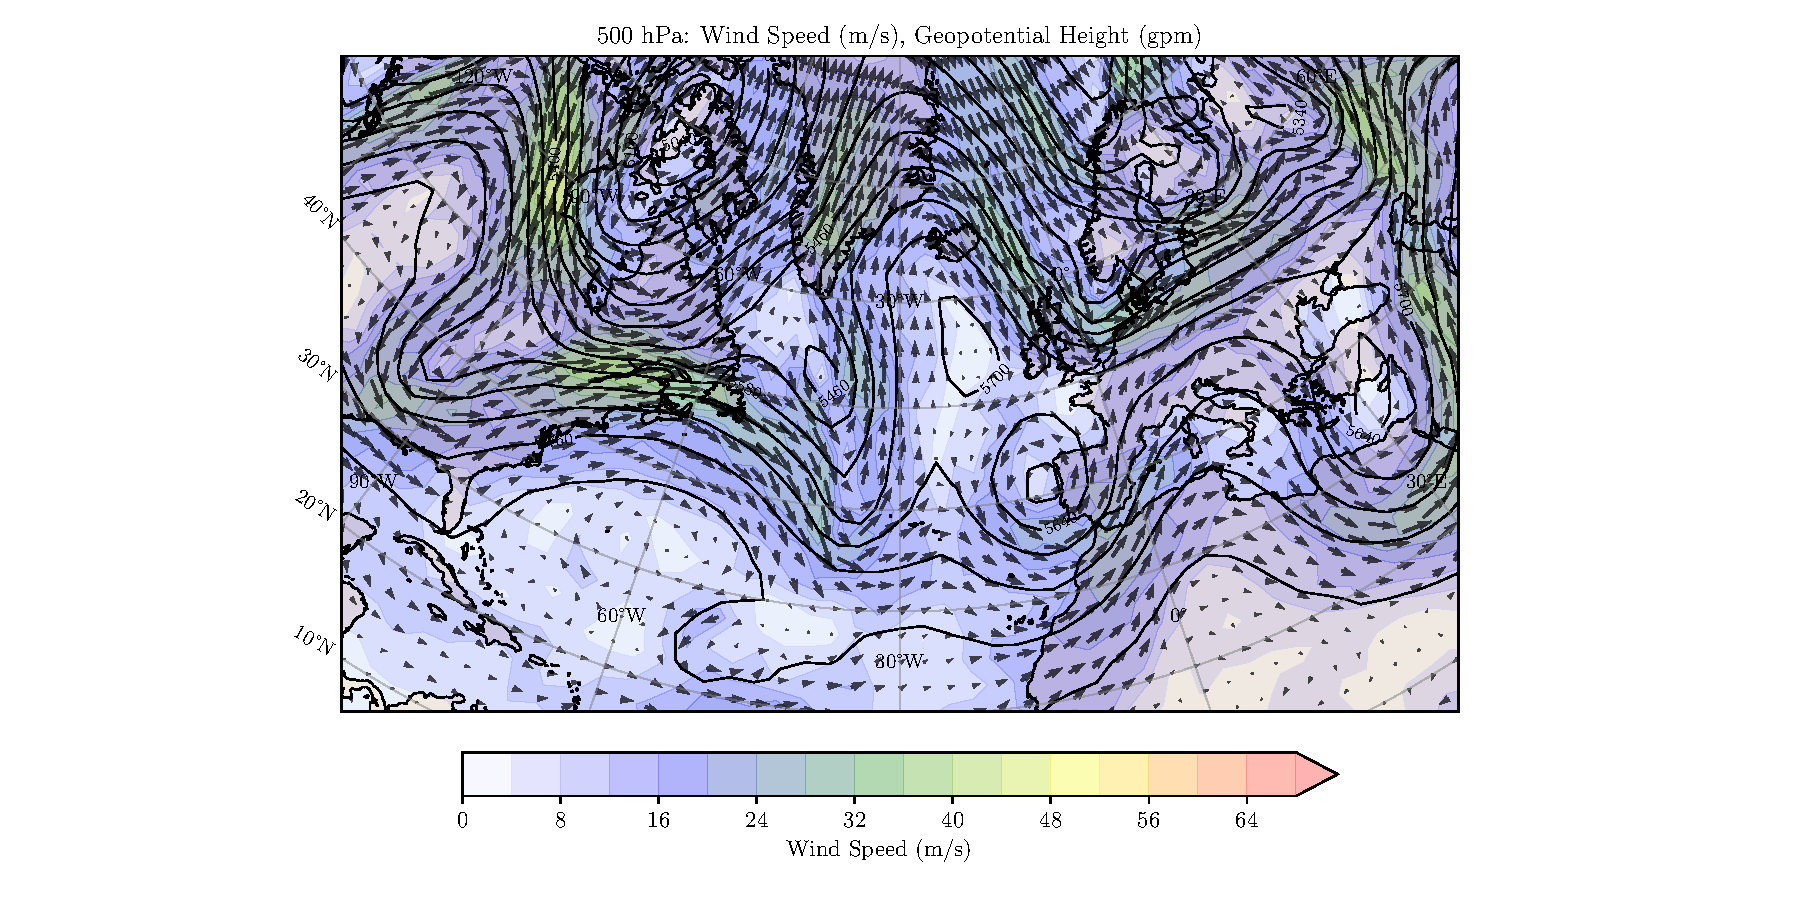
\includegraphics[width=0.32\textwidth, trim=5cm 0cm 5cm 0cm, clip]{papers/rossby/images/weather/data_2025_5_3_12:00_500.pdf} \\
            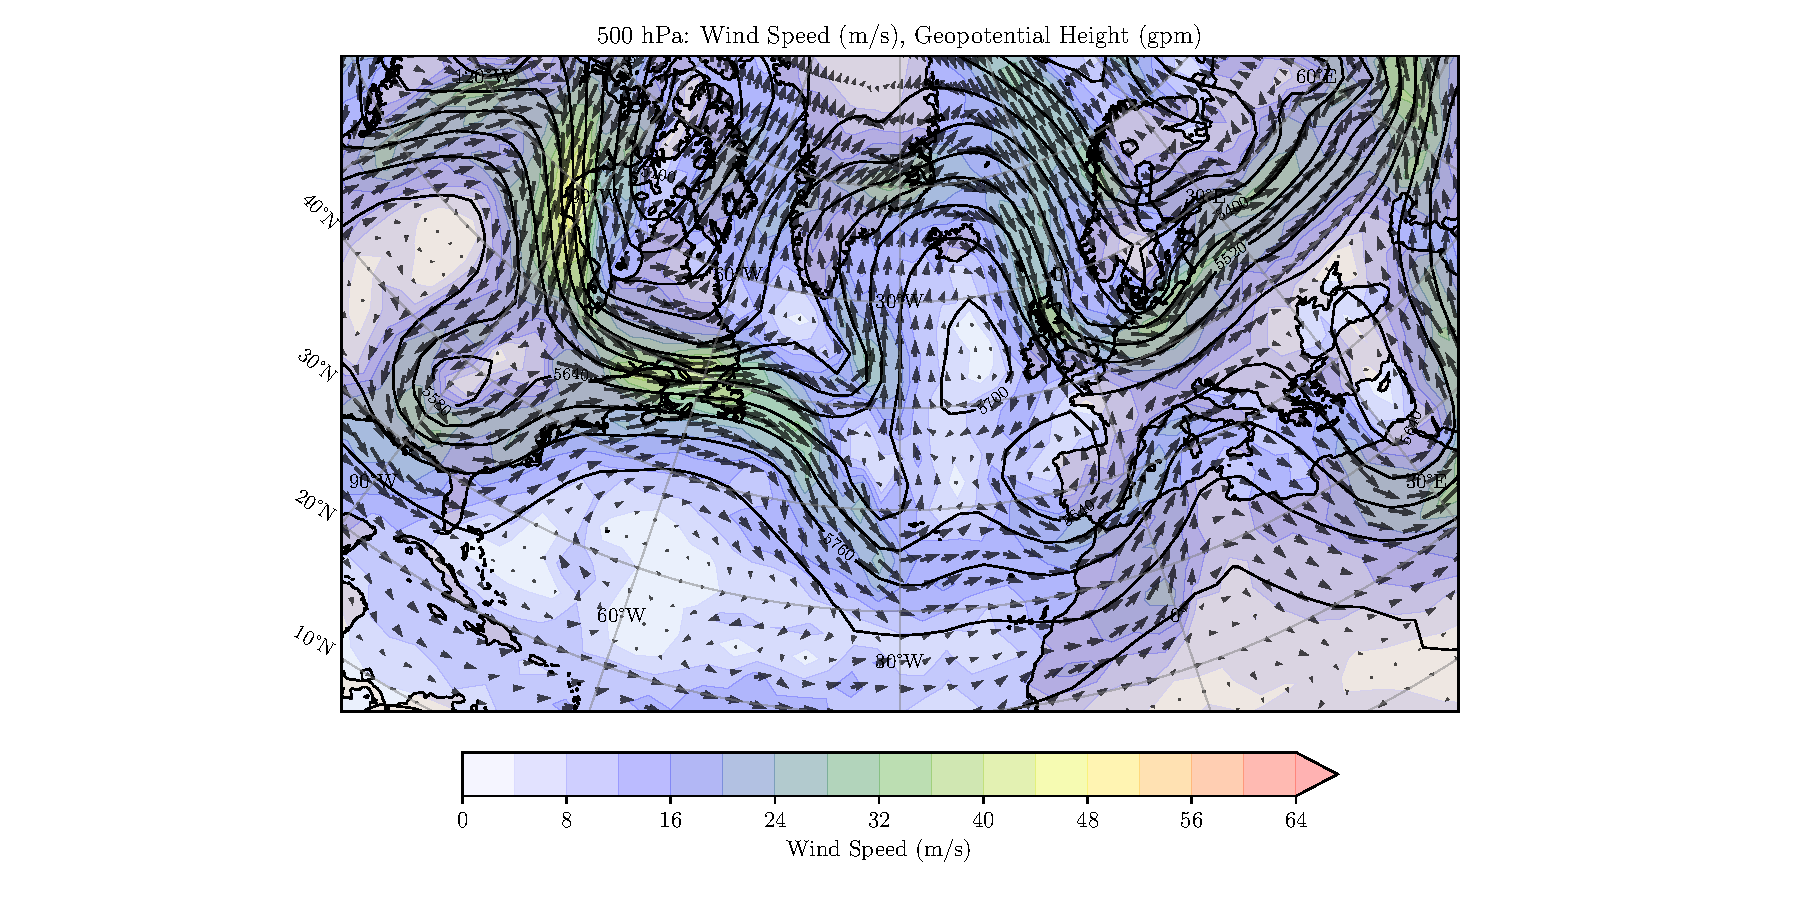
\includegraphics[width=0.32\textwidth, trim=5cm 0cm 5cm 0cm, clip]{papers/rossby/images/weather/data_2025_5_4_00:00_500.pdf} &
            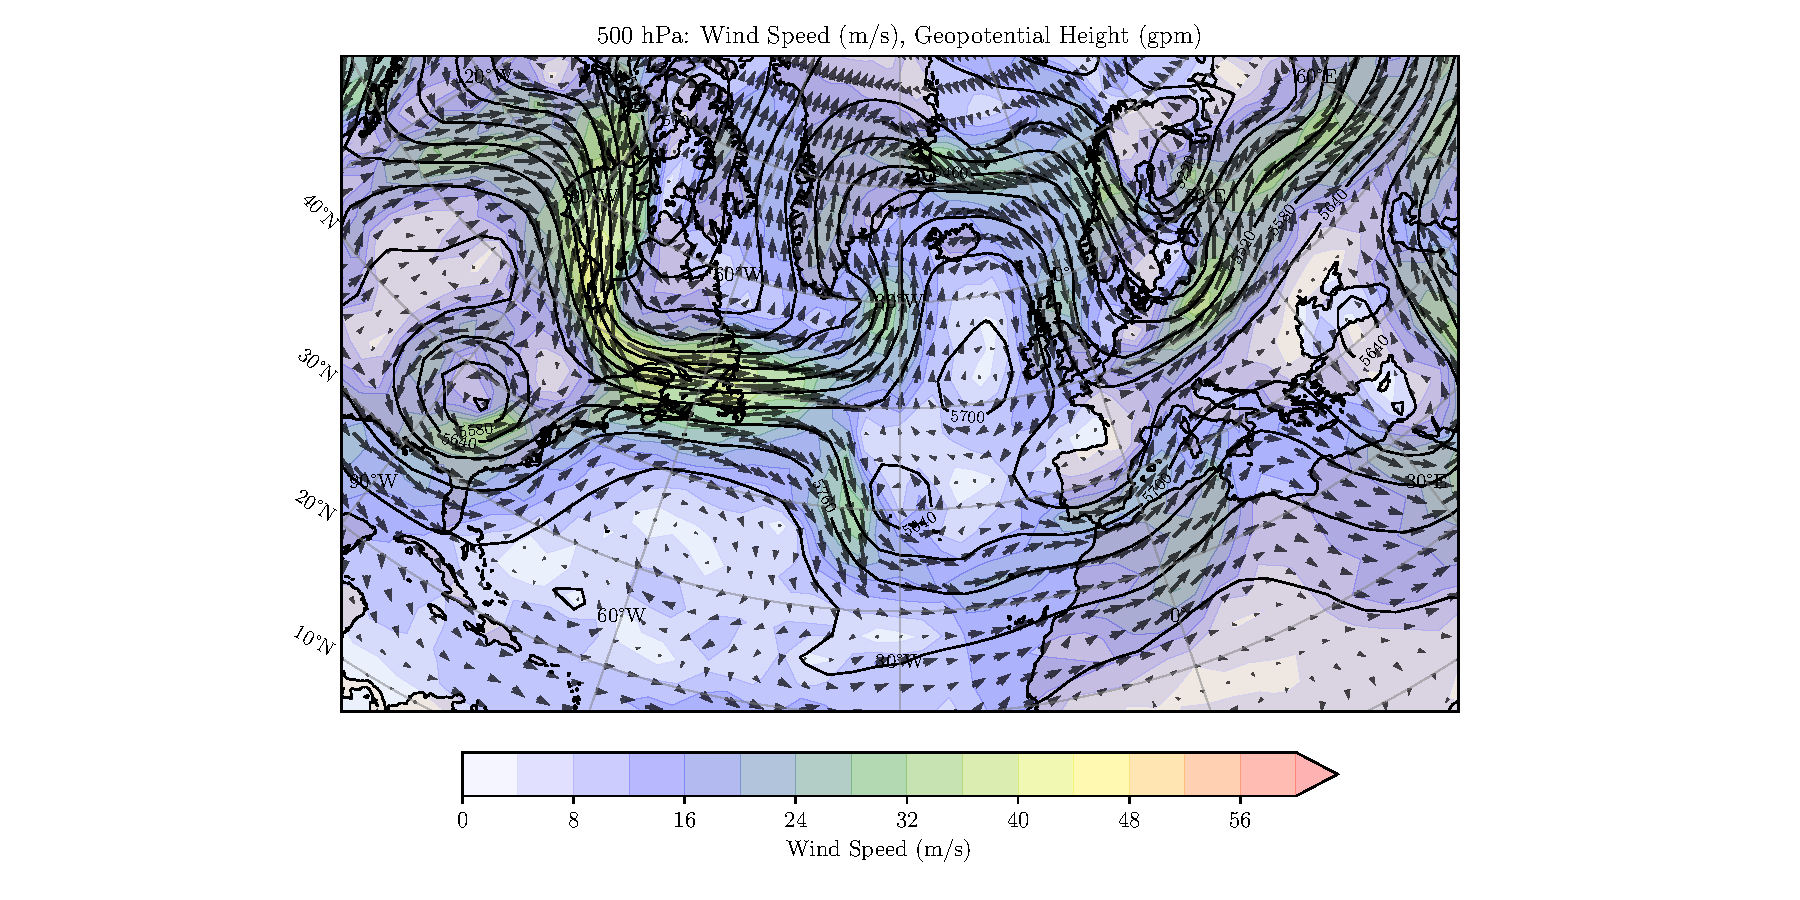
\includegraphics[width=0.32\textwidth, trim=5cm 0cm 5cm 0cm, clip]{papers/rossby/images/weather/data_2025_5_4_12:00_500.pdf} &
            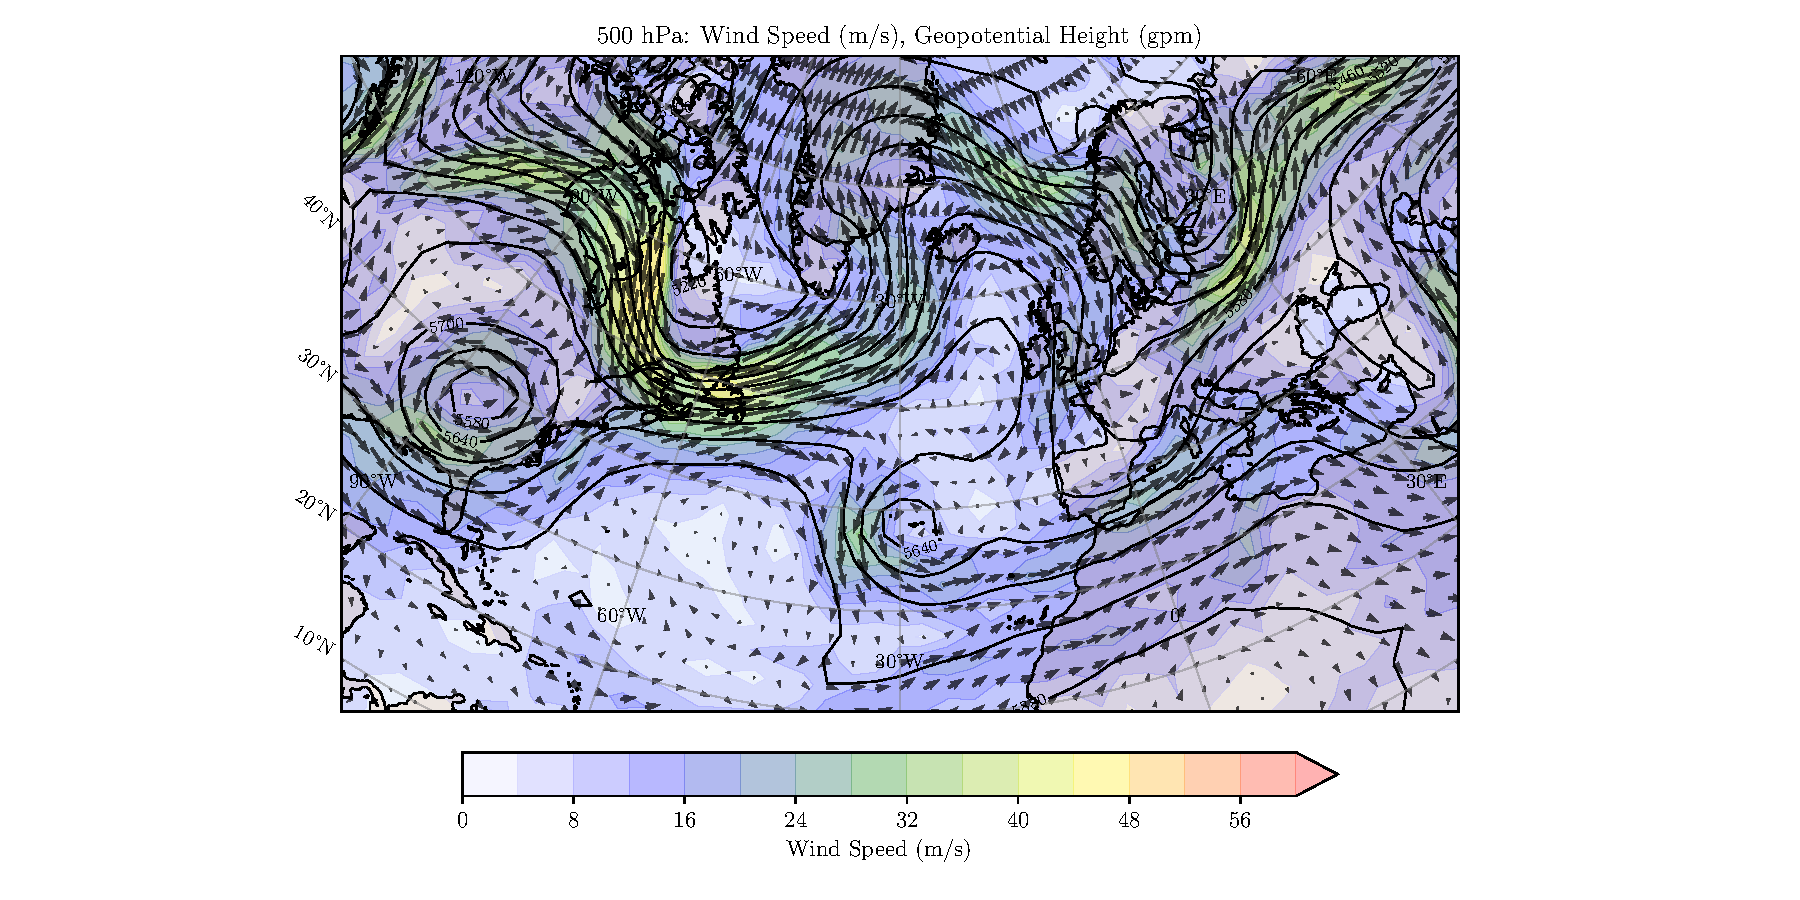
\includegraphics[width=0.32\textwidth, trim=5cm 0cm 5cm 0cm, clip]{papers/rossby/images/weather/data_2025_5_5_00:00_500.pdf} \\
        \end{tabular}
        \caption{Rossby-Wellenstruktur auf dem 500\,hPa-Niveau im Zeitraum 1.-5. Mai 2025. Wellenbewegung von West nach Ost ist deutlich erkennbar.}
        \label{fig:rossby_grid}
    \end{figure}
    

    \section{Die Drehung der Erde und der Coriolis-Effekt}

    Die Erde rotiert einmal pro Tag um ihre eigene Achse, was eine Vielzahl dynamischer Effekte in der Atmosphäre zur Folge hat.  
    In einem rotierenden Bezugssystem wie der Erde treten sogenannte Trägheits- oder Scheinkräfte auf, die in der klassischen Mechanik berücksichtigt werden müssen.  
    Eine dieser Kräfte ist die \emph{Coriolis-Kraft}, die bewirkt, dass bewegte Luftmassen auf der Nordhalbkugel nach rechts und auf der Südhalbkugel nach links abgelenkt werden.  
    Diese Ablenkung ist keine tatsächliche Kraft, sondern eine Folge der Drehung des Koordinatensystems.  
    
    Die Stärke der Coriolis-Kraft hängt von der geographischen Breite und der Geschwindigkeit der Bewegung ab.  
    Mathematisch wird sie durch den Term $-2\vec{\Omega} \times \vec{v}$ beschrieben, wobei $\vec{\Omega}$ der Vektor der Erdrotation und $\vec{v}$ die Geschwindigkeit der Luftmasse ist.  
    In atmosphärischen Anwendungen wird häufig nur die Vertikalkomponente betrachtet, was zur Definition des sogenannten \emph{Coriolis-Parameters} $f = 2\Omega \sin \varphi$ führt.  
    Dieser Parameter spielt eine zentrale Rolle in der grossräumigen Dynamik, insbesondere bei der Herleitung der geostrophischen und quasi-geostrophischen Gleichungen.  
    
    Die Coriolis-Kraft führt dazu, dass Luftmassen nicht direkt vom Hoch- zum Tiefdruckgebiet strömen, sondern entlang der Isobaren gelenkt werden.  
    Dieser Effekt ist massgeblich verantwortlich für das Auftreten von Westwinden in den mittleren Breiten sowie für die Entstehung grossskaliger Zirkulationssysteme.  
    Er bildet damit die physikalische Grundlage für die Entstehung von Rossby-Wellen.  
    
    \section{Vorticity - Wirbelstärke in der Atmosphäre}

    Die großräumige Bewegung der Luft in der Atmosphäre lässt sich nicht nur durch Geschwindigkeit beschreiben, sondern auch durch ihre Rotationseigenschaften.  
    Diese Eigenschaft wird durch die sogenannte \emph{Vorticity} (Wirbelstärke) quantifiziert.  
    Physikalisch beschreibt sie die Tendenz eines Luftpakets, sich um seine eigene vertikale Achse zu drehen.  
    
    Mathematisch ist die Vorticity definiert als Rotation des Geschwindigkeitsfeldes:  
    \[
    \vec{\zeta} = \nabla \times \vec{v}
    \]  
    Für großräumige Strömungen in der Atmosphäre betrachtet man hauptsächlich die vertikale Komponente dieser Rotation, die sogenannte \emph{relative Vorticity}.  
    In kartesischen Koordinaten ergibt sich diese im einfachsten Fall zu:
    \[
    \zeta = \frac{\partial v}{\partial x} - \frac{\partial u}{\partial y}
    \]
    wobei \( u \) und \( v \) die zonale bzw. meridionale Windkomponente bezeichnen.  
    
    Positive Vorticity bedeutet eine zyklonale (auf der Nordhalbkugel gegen den Uhrzeigersinn), negative eine antizyklonale Rotation.  
    Regionen hoher Vorticity sind oft mit Tiefdruckgebieten und dynamisch aktiven Wetterzonen assoziiert.  
    Die Vorticity ist eine zentrale Größe zur Beschreibung der atmosphärischen Dynamik, insbesondere in der quasi-geostrophischen Theorie.  
    Sie bildet zudem die Grundlage für die Einführung der \emph{absoluten} und \emph{potenziellen} Vorticity in den folgenden Abschnitten.  
    
    \section{Absolute Vorticity}

    Die bisher betrachtete relative Vorticity beschreibt die Rotation eines Luftpakets relativ zum Erdboden.  
    Da sich jedoch auch die Erde selbst dreht, muss diese planetare Rotation bei der Beschreibung der Gesamtdrehung berücksichtigt werden.  
    Daraus ergibt sich der Begriff der \emph{absoluten Vorticity}, welche die Summe aus relativer und planetarer Vorticity darstellt.  
    
    Die planetare Vorticity wird durch den sogenannten \emph{Coriolis-Parameter} \( f = 2 \Omega \sin \varphi \) beschrieben, wobei \( \Omega \) die Erdrotationsrate und \( \varphi \) die geographische Breite ist.  
    Dieser Ausdruck ergibt sich aus der Projektion der Erdrotation auf die lokale Vertikale.  
    Die absolute Vorticity ergibt sich somit zu:
    \[
    \eta = \zeta + f
    \]
    wobei \( \zeta \) die relative und \( f \) die planetare Vorticity ist.  
    
    Die absolute Vorticity ist eine Erhaltungsgröße in der reibungsfreien, barotropen Atmosphäre, wenn keine vertikalen Bewegungen stattfinden.  
    Sie spielt daher eine zentrale Rolle in der dynamischen Meteorologie und bildet die Grundlage für das Konzept der \emph{potenziellen Vorticity}, welches zusätzlich die Schichtung der Atmosphäre berücksichtigt.  
    
    \section{Potenzielle Vorticity und ihre Erhaltung}

Die potenzielle Vorticity (PV) erweitert das Konzept der absoluten Vorticity um die vertikale Struktur der Atmosphäre.  
Sie ist insbesondere in der Erhaltungsform ein mächtiges Werkzeug zur Beschreibung großskaliger Strömungen und Wellenerscheinungen.  

Unter vereinfachten Bedingungen - barotrope, reibungsfreie Atmosphäre mit konstantem Luftvolumen - ergibt sich die potenzielle Vorticity als:
\[
q = \frac{\zeta + f}{H}
\]
Dabei bezeichnet \( \zeta \) die relative Vorticity, \( f \) den Coriolis-Parameter, und \( H \) die effektive Schichthöhe der Atmosphäre.  
Dieser Ausdruck berücksichtigt sowohl die Rotation als auch die vertikale Ausdehnung eines Luftpakets.  

Ein zentrales Ergebnis der quasi-geostrophischen Theorie ist die Erhaltung der potenziellen Vorticity entlang der Trajektorie eines Luftpakets:
\[
\frac{Dq}{Dt} = 0
\]
Diese Gleichung besagt, dass sich \( q \) nur verändert, wenn entweder äußere Kräfte (z.B. Reibung oder diabatische Prozesse) eingreifen oder sich die Schichthöhe \( H \) durch vertikale Bewegung ändert.  

Die PV-Erhaltung erklärt viele großskalige atmosphärische Phänomene:  
Wenn ein Luftpaket nach Norden (größeres \( f \)) bewegt wird, muss es zyklonale Vorticity (\( \zeta > 0 \)) verlieren oder sich ausdehnen (\( H \uparrow \)), um \( q \) konstant zu halten.  
Analog verhält es sich bei südlicher Verlagerung.  
Diese Mechanismen bilden die physikalische Grundlage für die Rossby-Wellen, die im nächsten Kapitel beschrieben werden.  

\section{Rossby-Wellen - Entstehung und Eigenschaften}

Rossby-Wellen, auch planetare Wellen genannt, sind großräumige Wellenerscheinungen, die in erster Linie durch die Änderung des Coriolis-Parameters mit der Breite verursacht werden.  
Diese Breitenabhängigkeit wird durch den sogenannten \emph{Beta-Term} beschrieben:
\[
\beta = \frac{\partial f}{\partial y}
\]
Sie führt dazu, dass Luftpakete bei meridionaler Bewegung eine Änderung ihrer planetaren Vorticity erfahren, was - unter der Erhaltung der potenziellen Vorticity - eine Reaktion der Strömung erzwingt.  

Die Rossby-Welle ist also eine direkte Konsequenz der PV-Erhaltung auf einer Kugel oder Beta-Ebene.  
Ihre typische Wellenform entsteht, wenn ein Luftpaket nach Norden oder Süden ausgelenkt wird und dabei durch die Änderung von \( f \) eine kompensierende Änderung von \( \zeta \) erfahren muss.  
Dies führt zu einer wellenförmigen Rückstellbewegung, die sich nach Westen ausbreitet.  

Die einfachste theoretische Form einer barotropen Rossby-Welle ergibt sich aus der linearen Wellengleichung:
\[
c = u - \frac{\beta}{k^2}
\]
Hierbei ist \( c \) die Phasengeschwindigkeit, \( u \) die mittlere Strömungsgeschwindigkeit, \( \beta \) der Gradient des Coriolis-Parameters, und \( k \) die Wellenzahl.  
Daraus folgt, dass sich Rossby-Wellen relativ zur Strömung immer nach Westen ausbreiten.  
In der Erdatmosphäre bedeutet das: Obwohl die Luftströmung nach Osten gerichtet ist (z.B. Jetstream), propagiert die Wellenform gegen die Strömung.  

Rossby-Wellen sind besonders stabil und können über viele Tage bestehen bleiben.  
Sie beeinflussen großräumig die Lage und Bewegung von Hoch- und Tiefdrucksystemen sowie die Pfade von Wetterfronten.  
Damit spielen sie eine entscheidende Rolle für die mittelfristige Wetterentwicklung in den mittleren Breiten.

\section{Rossby-Wellen und Wetterextreme: Der Sommer 2010}

Ein eindrucksvolles Beispiel für den Einfluss quasi-stationärer Rossby-Wellen auf Extremwetterereignisse ist der Sommer 2010.  
In diesem Zeitraum traten gleichzeitig zwei außergewöhnliche Wetterlagen auf, die durch eine wellenartige atmosphärische Zirkulationsstruktur mit Wellenzahl \( k = 7 \) verursacht wurden.  

Über Russland bildete sich ein stabiles Hochdruckgebiet, das eine extreme Hitzewelle mit Temperaturen über 40\,$^\circ$C verursachte.  
Infolge der langanhaltenden Trockenheit kam es zu großflächigen Waldbränden und Smog in der Region Moskau, mit tausenden Todesopfern.  

Gleichzeitig wurde Pakistan von ungewöhnlich starkem Monsunregen heimgesucht.  
Ein quasi-stationäres Tiefdrucksystem führte zu einer Jahrhundertflut, die über 20 Millionen Menschen betraf.  

Beide Ereignisse lassen sich durch dieselbe planetare Wellenstruktur erklären:  
Die quasi-stationäre Rossby-Welle führte zu einem blockierenden Hoch über Russland und einem persistenten Tief über Pakistan.  

Dieses Beispiel zeigt deutlich, wie großskalige Dynamik auf der planetaren Skala direkte Auswirkungen auf regionale Extremwetterlagen haben kann.  
Es unterstreicht die Bedeutung von Rossby-Wellen in der Wetter- und Klimadynamik.\cite{rossby:petoukhov2013}


	\printbibliography[heading=subbibliography]
\end{refsection}
